\section{Modelos Matemáticos para Sistemas Continuos}

\begin{frame}{Categorías de variables y constantes}
    \begin{itemize}
        \item<1-> \textbf{Constante:} una cantidad en el modelo que no varía nunca, por ejemplo la gravedad en la tierra $g=9.8$.
        \item<2-> \textbf{Parámetro de modelo:} una constante en el modelo que es determinada por el sistema, o una constante que puede ser modificada con el fin de darle diferentes propiedades al sistema. Permance constante durante la simulación pero puede ser modificado entre ejecuciones.
        \item<3-> \textbf{Variable:} una cantidad en el modelo que varia respecto del tiempo.
    \end{itemize}
\end{frame}

\begin{frame}{Categorías de variables y constantes}
    \begin{itemize}
        \item<1-> \textbf{Variable de salida:} una variable cuyo comportamiento queremos observar. Usualmente denotada como $y(t)$. El rol de variable de salida no está establecido por el sistema que se modela sino que es determinado por lo que el modelador quiere estudiar.
        \item<2-> \textbf{Variable de entrada:} una variable que afecta el comportamiento del modelo sin ser afectada por otras variables del modelo y cuyas variaciones respecto del tiempo pueden ser controladas. Usualmente se las denota $u(t)$.
        \item<3-> \textbf{Variable de estado}: una variable que no es ni de entrada ni de salida y que aparece su derivada respecto del tiempo, usualmente denotada por $\dot{x}(t)$
        \item<4-> \textbf{Variables algebraicas:} una variable que aparece en las ecuaciones pero que su derivada no aparece en el modelo.
    \end{itemize}
\end{frame}

\begin{frame}{Ecuacion diferencial ordinaria en forma de espacio de estados explícita}

    \note{ Las ecuaciones diferenciales ordinarias aparecen en la mayoría de los modelos matemáticos de sistemas continuos dado que la dependencia respecto del tiempo en esos modelos generalmente se refleja por medio de derivadas respecto del tiempo de variables de estado correspondientes a dichos modelos.\\
    Un modelo ODE de espacio de estados explícito resulta más eficiente de resolver y analizar que otros modelos más complicados. }

    \begin{block}{Forma general}
        \begin{align*}
            \dot{x}(t) & =f(x(t),u(t)) \\
            y(t)       & =g(x(t),u(t))
        \end{align*}
    \end{block}
    \begin{block}{Ejemplo: Ley de fuerza de Newton}
        $m\ddot{s}(t)=F(t)$\\
        \pause
        \begin{align*}
            \dot{v}(t) & =\frac{F(t)}{m}\\
            \dot{s}(t) & =v(t)
        \end{align*}
    \end{block}
\end{frame}

\begin{frame}[fragile]{Ecuacion diferencial algebraica}
   \framesubtitle{Ejemplo: Péndulo Plano} 
    \note{Cinco de las ecuaciones del modelo son diferenciales y dos son algebraicas.
        Las variables del modelo son $x$, $y$, $v_{x}$, $v_{y}$, $\varphi$,
        $\omega$, $F$ y las constantes $L$, $m$, $g$. Hemos reemplazado
        la ecuación correspondiente a la ley de Pitagóras por dos ecuaciones
        algebraicas sobre las variables $x$ e $y$ respectivamente, las cuales
        aún preservan la restricción sobre la longitud del péndulo.}
    \begin{columns}
        \begin{column}{0.5\textwidth}
            \begin{figure}
              \centering
              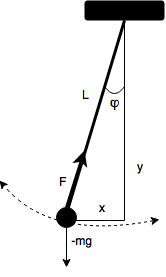
\includegraphics[width=0.5\textwidth]{graphics/pendulum.png}
            \end{figure}
        \end{column}
        \begin{column}{0.5\textwidth}
            \begin{align*}
                m\dot{v_{x}}  & =-F\sin(\varphi)\nonumber \\
                m\dot{v_{y}}  & =-F\cos(\varphi)-mg\nonumber \\
                \dot{x}       & =v_{x}\nonumber \\
                \dot{y}       & =v_{y}\label{eq:pendulo}\\
                \dot{\varphi} & =\omega\nonumber \\
                x             & =L\sin(\varphi)\nonumber \\
                y             & =-L\cos\left(\varphi\right)\nonumber
            \end{align*} 
        \end{column}
    \end{columns}
\end{frame}

\begin{frame}[fragile]{Ecuacion diferencial algebraica}
   
   \note{ Las ecuaciones diferenciales algebraicas no son los modelos más eficientes para resolver ya que las derivadas no siempre aparecen del lado izquierdo y por lo tanto puede ser necesario aplicar derivación numérica }

   \begin{block}{Forma General}
       \begin{align*}
            F(x(t),\dot{x}(t),u(t),y(t)) & =0 \\
            G(x(t),u(t),y(t))            & =0
       \end{align*}
    \end{block}
\end{frame}




